\scanpage{105}

\margin{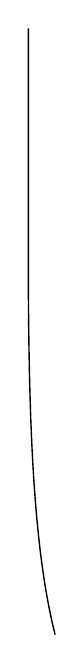
\begin{tikzpicture}\draw[line width=0.5pt] (0,7.7)--(0,4.4).. controls (0.01,2.7) and (0.06,1.1) .. (0.34,0);\end{tikzpicture}}
\textcircled{4} By the pairing \deleted{\unsure{of}}

\[
\langle u,v\rangle=\operatorname{Tr}vu\tag*{\textcircled{26}}
\]

the dual of $L_N(E,F)$ is identified with $L^{N^\circ}(F,E)$. If $E$ and $F$ are infinite-dimensional, \deleted{\unsure{the following spaces|the two conditions} $L_N(E,F)$} \inserted{then} following conditions are equivalent\,: a) $L_N(E,F)$ is reflexive \deleted{$L_N(E,F)=L^N(E,F)$ and $L_{N^\circ}(F,E)=L^{N^\circ}(\unsure{F|F,E})$} b) $L^N(E,F)$ is reflexive c) $\ell^{\deleted{\unsure{\ell|N}}}_{N}$ is reflexive \deleted{\unsure{f),}} d) $\ell_{N'}$ is reflexive. \deleted{\unsure{it is and only if}, \unsure{$\ell$} \unsure{equivalent of these propositions to}\,: d) $\ell^N$ is reflexive. -- e) $\ell_{N^\circ}$ is reflexive and \unsure{finally} f) $\ell^{N^\circ}$ is reflexive)} \deleted{\unsure{then}} d) $L_N(E,F)=L^N(E,F)$ and $\begin{aligned}&L_{N^\circ}(F,E)=L^{N^\circ}(F,E)\\[-0.5ex]&\quad\text{\deleted{\unsure{and}}}\end{aligned}$

\textcircled{5} \deleted{\unsure{Let us note|Remark}} Let $u\in L_0(E,F)$, \deleted{if $u\in L^N(E,\unsure{F|E})$\unsure{,} \unsure{then} \unsure{Then} $(\lambda_i(u))\in\ell^N$,} \inserted{Then}

\[
N((\lambda_i(u)))\leq\deleted{N(\unsure{(\rho_i(u))|(\rho_i u)})}N(u)\tag*{(27)}
\]

If $u\in L^N(E,F)$, \deleted{then (respectively $L_N(E,E)$)} then, $(\lambda_i(u))\in\deleted{\unsure{\ell_N|L^N\unsure{,}|\ell^N}}\ell^N$ \deleted{(respectively $\ell_N$)}

Everything is proved, except 4. \deleted{\unsure{and}} and 5. For 4, we note\,: if $E$ and $F$ are infinite-dimensional, then $\ell^N$ \inserted{(respectively $\ell_N$)} is isometric to a normed vector subspace of $L^N(E,F)$ (respectively $L_N(E,F)$. (\textcolor{red}{\uline{\textcolor{black}{take}}} $(e_i)$, $(f_i)$ infinite orthonormal systems, and $(\lambda_i)\to\sum\lambda_i\bar e_i\otimes f_i$ from $\ell^N$ into $L^N(E,F)$). \deleted{Therefore}

If $L^N_{\deleted{\unsure{0|N}}}(E,F)$ is reflexive, $L_N(E,F)$ is reflexive, and then also $\ell_N$ is reflexive, \deleted{\unsure{therefore}}\inserted{\unsure{This|which} implies} (see --) $\ell_N=\ell^N$, $\ell_{N^\circ}=\ell^{N^\circ}$, therefore $L^N(E,F)=L_N(E,F)$ (for we \deleted{\unsure{can assume}}\inserted{will have} required $N\unsure{\not\simeq|\neq}N_\infty$), therefore $L^N(E,F)$ will be reflexive, whence the equivalence a), b), c).

\margin{
\begin{tikzpicture}\draw[red,line width=0.65pt] (0,2.35).. controls (0.09,1.55) and (0.10,0.75) .. (0.19,0.48);\draw[red,line width=0.45pt] (0.04,1.34).. controls (0.02,0.79) and (0.07,0.31) .. (0.12,0);\end{tikzpicture}}
And the fact that this implies d) (first the first assertion, for the second we $\ell_{N^\circ}$ will also be reflexive). Finally d implies \deleted{$\ell_N=\ell^N$ and $\ell_{N^\circ}=\ell^{N^\circ}$ (see \unsure{previous theorem|previous theorem}) therefore $\ell_N$ reflexive (\unsure{always|see --})} \inserted{that the dual of $L_N(E,F)$ is $L_{N^\circ}(F,E)$,} whose dual is $L_N(E,F)$, therefore $L_N(E,R)$ is reflexive.

\textcircled{5} (27) Is corollary 5 of the 1. convexity theorem \deleted{\unsure{Follows at once from the|follows immediately}}
\margin{106}
